\problemname{Geometric Gridlock}

\emph{Pentominous} is a grid logic puzzle based on the twelve pentominoes. A pentomino is a polygon formed by connecting five equal-sized squares edge to edge.

\begin{figure}[!h]
  \centering
  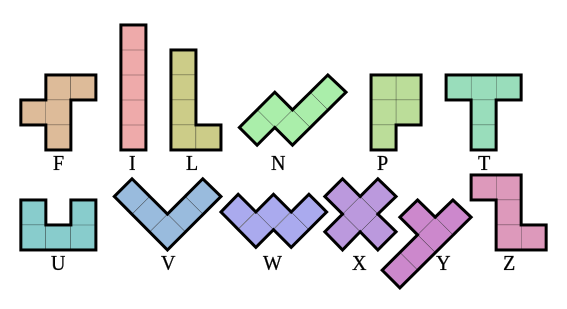
\includegraphics[width=0.6\textwidth]{pentominoes}
  \caption{The twelve pentominoes (up to mirroring and rotations) and their names.}
  \label{fig:pentominoes}
\end{figure}

The goal of this puzzle is to divide a grid into regions of size $5$ (that is, pentominoes), so that no two regions that share a side have the same shape.
You are allowed to rotate and mirror the pentominoes, but such rotations and reflections count as the same shape.
The twelve possible shapes can be seen in Figure~\ref{fig:pentominoes}.

In a normal \emph{Pentominous} puzzle, the player is given some pre-filled cells, for which the shape of their region is already predetermined.
In this problem, you are working with a completely blank grid of dimensions $h\times w$, and your task is to create any valid arrangement of pentominoes.

\begin{Input}
  The input consists of:
  \begin{itemize}
    \item One line with two integers $h$ and $w$ ($1 \le h,w \le 100$), the height and width of the grid.
  \end{itemize}
\end{Input}

\begin{Output}
  If there is no valid $h\times w$ \emph{Pentominous} grid, output ``\texttt{no}''.
  Otherwise, output ``\texttt{yes}'', followed by $h$ lines of width $w$ each, a possible grid using the letters from Figure~\ref{fig:pentominoes}.
  If there is more than one solution, any one of them will be accepted.
\end{Output}
